%% ------------------------------------------------------------------------- %%n
\chapter{Plano de Trabalho e Cronograma}
\label{cap:Cronogramanotes}

\NINA{Neste capítulo apresentamos uma breve descrição das atividades já realizadas e um plano de trabalho juntamente com um cronograma.}

Os créditos em disciplinas requeridos pelo programa de mestrado em Ciência da Computação
no IME-USP foram cumpridos de fevereiro de 2016 até junho de 2018, conforme a tabela a seguir: 

\begin{center}
\begin{tabular}{ |l|l|l| } 
\hline
\textbf{Código} & \textbf{Disciplina}                                   & \textbf{Término} \\ 
\hline
MAC5710     & Estrutura de Dados e sua Manipulação (Aluno Especial)     & 10/06/2016       \\
MAC4722     & Linguagens, Autômatos e Computabilidade                   & 30/06/2017       \\
MAC6910     & Metodologia de Pesquisa para Ciência da Computação        & 30/06/2017       \\
MAC5749     & Análise e Reconhecimento de Formas: Teoria e Prática      & 24/11/2017       \\
MAC5861     & Modelagem de Banco de Dados                               & 24/11/2017       \\
MAC5832     & Aprendizagem de Máquina: Modelos, Algoritmos e Aplicações & 22/06/2018       \\
\hline
\end{tabular}
% \label{tab:disciplinas}
\end{center}

\NINA{Além do estudo bibliográfico (conteúdo apresentado no capítulo 2) para aquisição de conhecimentos sobre os fundamentos do aprendizado ativo assim como desenvolvimentos mais recentes relacionados a esse tópico, foi realizada familiarização com as imagens de plâncton, e também alguns experimentos preliminares para fixação de conceitos de aprendizado de máquina e de aprendizado ativo (capítulo~\ref{cap:Experimentos_Resultados}). Todas essas atividades foram importantes para a delineação da proposta (capítulo~\ref{cap:Proposta}) e do plano de trabalho descrito a seguir.}


\section{Plano de Trabalho}
\label{sec:Plano_de_Trabalho}

As principais atividades planejadas para a conclusão do trabalho proposto são:

\begin{enumerate}
  \item Estudo complementar de trabalhos existentes sobre a participação ativa de usuários em contextos relacionados a aprendizado ativo. Alguns trabalhos que exploram, por exemplo, a visualização dos dados como mecanismo de interação do usuário foram descritos no texto e deverão ser estudados de forma aprofundada;  
  
  \item Desenvolvimento de mecanismos de participação ativa do usuário em  frameworks de aprendizado ativo. Especificamente, espera-se desenvolver mecanismos que permitam ao usuário interagir de forma ativa no processo de aprendizado ativo. Por exemplo, a escolha das amostras a serem rotuladas em algumas iterações pode ser realizada pelo usuário;
  
  \item Implementação, teste e validação do método de aprendizado ativo com participação ativa do usuário. Os testes de implementação serão realizados com dados sintéticos ou subconjuntos dos datasets de plâncton considerados neste trabalho. A validação deverá ser realizada com os datasets de plâncton. Especificamente, a validação visa realizar uma comparação entre a seleção aleatória de amostras, o aprendizado ativo clássico (oráculo passivo) e o aprendizado ativo com atuação ativa de usuários (a ser desenvolvido neste trabalho). Essas comparações serão realizadas por meio de simulações usando as anotações disponíveis como oráculo. Neste sentido, precisaremos também definir como será simulada a interação ativa de usuários;
  
  \item Validação com usuários reais. Pretendemos também realizar uma validação com os membros do LAPS (Laboratório de Sistemas Planctônicos) do Instituto Oceanográfico da USP (IO-USP) em um caso real de classificação de um conjunto ainda não rotulado. Esta atividade será importante para uma avaliação qualitativa do método;
  
  \item Redação da dissertação e de artigos, e defesa do Mestrado.
\end{enumerate}


\section{Cronograma}
\label{sec:cronograma}


\begin{figure}
  \centering
  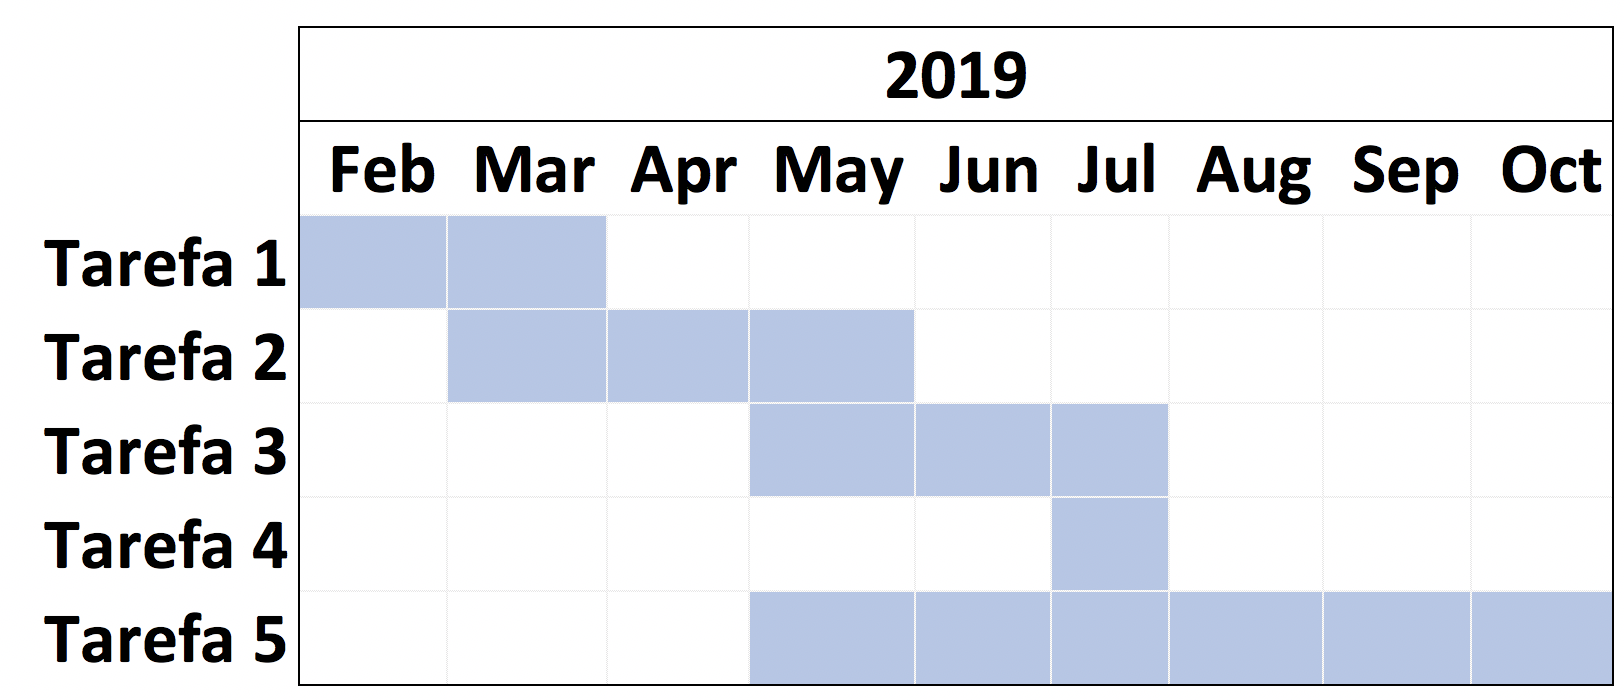
\includegraphics[width=0.6\textwidth]{figures/cronograma.png}
  \caption{Cronograma Mestrado.}
  \label{fig:cronograma}
\end{figure}
